\documentclass[aspectratio=169,10pt]{beamer}

\usepackage[T1]{fontenc}
\usepackage{lmodern}
\usepackage{microtype}
\usepackage{graphicx}
\usepackage{booktabs}
\usepackage{amsmath}
\usepackage{amssymb}
\usepackage{xcolor}
\usepackage{tikz}
\usepackage{pgfplots}
\pgfplotsset{compat=1.18}

% ── Theme ────────────────────────────────────────────────────────────
\usetheme{metropolis}
\usecolortheme{owl}
\setbeamercolor{normal text}{fg=white,bg=black!92!blue}
\setbeamercolor{alerted text}{fg=yellow!85!orange}
\setbeamercolor{frametitle}{bg=black!85!blue,fg=yellow!85!orange}
\setbeamercolor{progress bar}{fg=yellow!85!orange}
\setbeamercolor{title separator}{fg=yellow!85!orange}
\setbeamercolor{progress bar in head/foot}{fg=yellow!85!orange}
\setbeamercolor{progress bar in section page}{fg=yellow!85!orange}
\setbeamerfont{frametitle}{series=\bfseries}
\setbeamertemplate{itemize items}[circle]
\setbeamercovered{transparent=30}

% Stop a frame from being numbered (used for the title slide)
\makeatletter
\setlength{\metropolis@titleseparator@linewidth}{2pt}
\setlength{\metropolis@progressonsectionpage@linewidth}{1.5pt}
\setlength{\metropolis@progressinheadfoot@linewidth}{1.5pt}
\makeatother

% Suppress the auto-generated metropolis section page so we don't get
% blank dividers between every section in a 16:9 deck.
\AtBeginSection[]{}

% ── Title ────────────────────────────────────────────────────────────
\title{Real-Time Lane Detection \\ and Autonomous Steering}
\subtitle{A comparison of classical pipelines \\
  and a polynomial-fit improvement}
\author{David Tovmasyan}
\institute{Course project, May 2026}
\date{}

% ── Helpers ──────────────────────────────────────────────────────────
\newcommand{\highlight}[1]{\textcolor{yellow!85!orange}{\textbf{#1}}}
\newcommand{\code}[1]{\texttt{\small #1}}

\begin{document}

% ── Title slide ──────────────────────────────────────────────────────
\maketitle

% ── Outline ──────────────────────────────────────────────────────────
\begin{frame}{Where we are going}
  \small\tableofcontents
\end{frame}

% ════════════════════════════════════════════════════════════════════
\section{Motivation}
% ════════════════════════════════════════════════════════════════════

\begin{frame}{Why lane keeping (still) matters}
  \begin{columns}[T,onlytextwidth]
    \begin{column}{0.55\textwidth}
      \begin{itemize}
        \item Most-deployed AD function: every modern car ships
              lane-keep assist or adaptive cruise.
        \item Two coupled problems
              \begin{itemize}
                \item \highlight{Perception:} where is the lane?
                \item \highlight{Control:} how do we stay in it?
              \end{itemize}
        \item Learned segmenters dominate benchmarks, but a classical
              pipeline is:
              \begin{itemize}
                \item interpretable (debuggable),
                \item CPU-friendly ($>500$\,FPS),
                \item zero training data required.
              \end{itemize}
      \end{itemize}
    \end{column}
    \begin{column}{0.45\textwidth}
      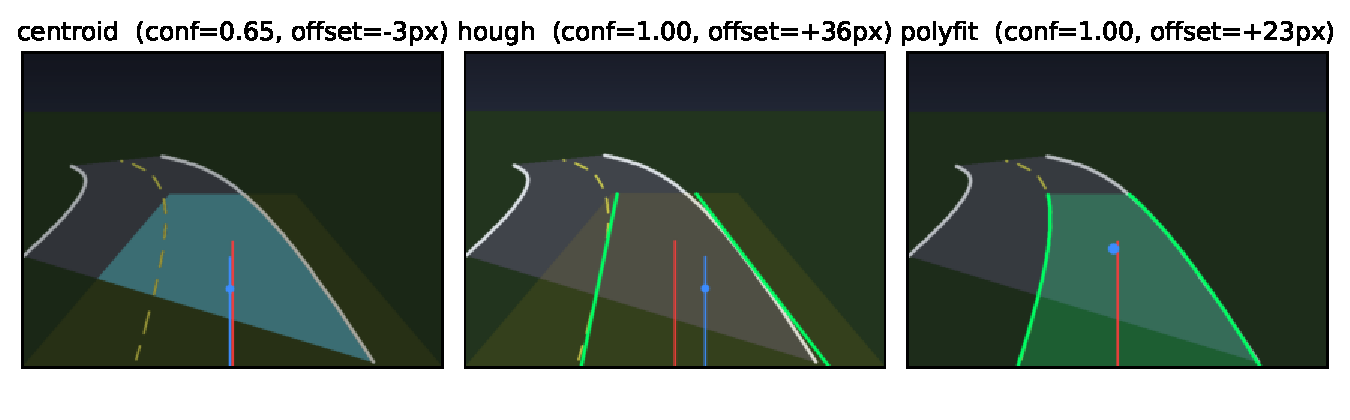
\includegraphics[width=\linewidth]{figures/annotations.pdf}\\
      {\footnotesize\color{gray}Same frame, three detectors.}
    \end{column}
  \end{columns}
\end{frame}

\begin{frame}{The concrete question}
  \begin{center}\Large
    How much performance is left on the table\\
    by the textbook Canny+Hough detector,\\
    and can a \highlight{polynomial-fit upgrade}\\
    close the gap on curved tracks\\
    while staying \highlight{real-time}?
  \end{center}
  \vspace{1em}
  \begin{itemize}
    \item Implement three classical methods of increasing sophistication.
    \item Plug each into a PID controller.
    \item Add a Stanley controller driven from \emph{ground truth} as a
          perception-free oracle (upper bound on what the controller
          can do given perfect perception).
    \item Evaluate on five tracks + a noise sweep.
  \end{itemize}
\end{frame}

% ════════════════════════════════════════════════════════════════════
\section{The simulator}
% ════════════════════════════════════════════════════════════════════

\begin{frame}{What we built}
  \begin{columns}[T,onlytextwidth]
    \begin{column}{0.55\textwidth}\footnotesize
      \begin{itemize}\setlength\itemsep{1pt}
        \item 2D forward-perspective driving simulator
              (Python + OpenCV + pygame).
        \item 5 tracks (difficulty 1--5), closed-loop Catmull--Rom
              spline.
        \item Camera: pinhole, $70^\circ$ FoV, $18^\circ$ pitch,
              $640\!\times\!480$ FPV.
        \item Vehicle: bicycle kinematics,
              $\dot\theta=(v/L)\tan\delta$.
        \item Three live panels: map, FPV overlay, dashboard.
      \end{itemize}
    \end{column}
    \begin{column}{0.43\textwidth}
      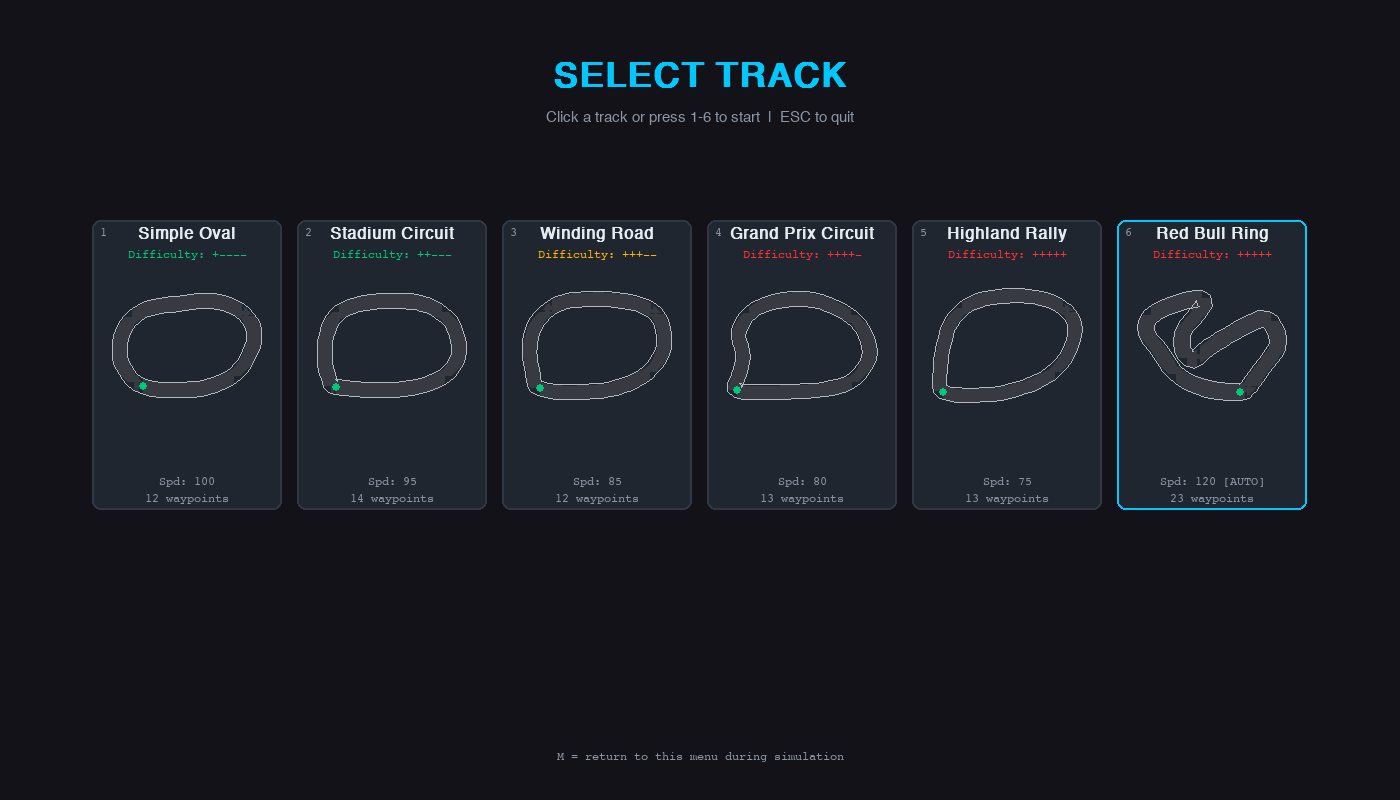
\includegraphics[width=\linewidth]{../docs/track_selector.png}\\[2pt]
      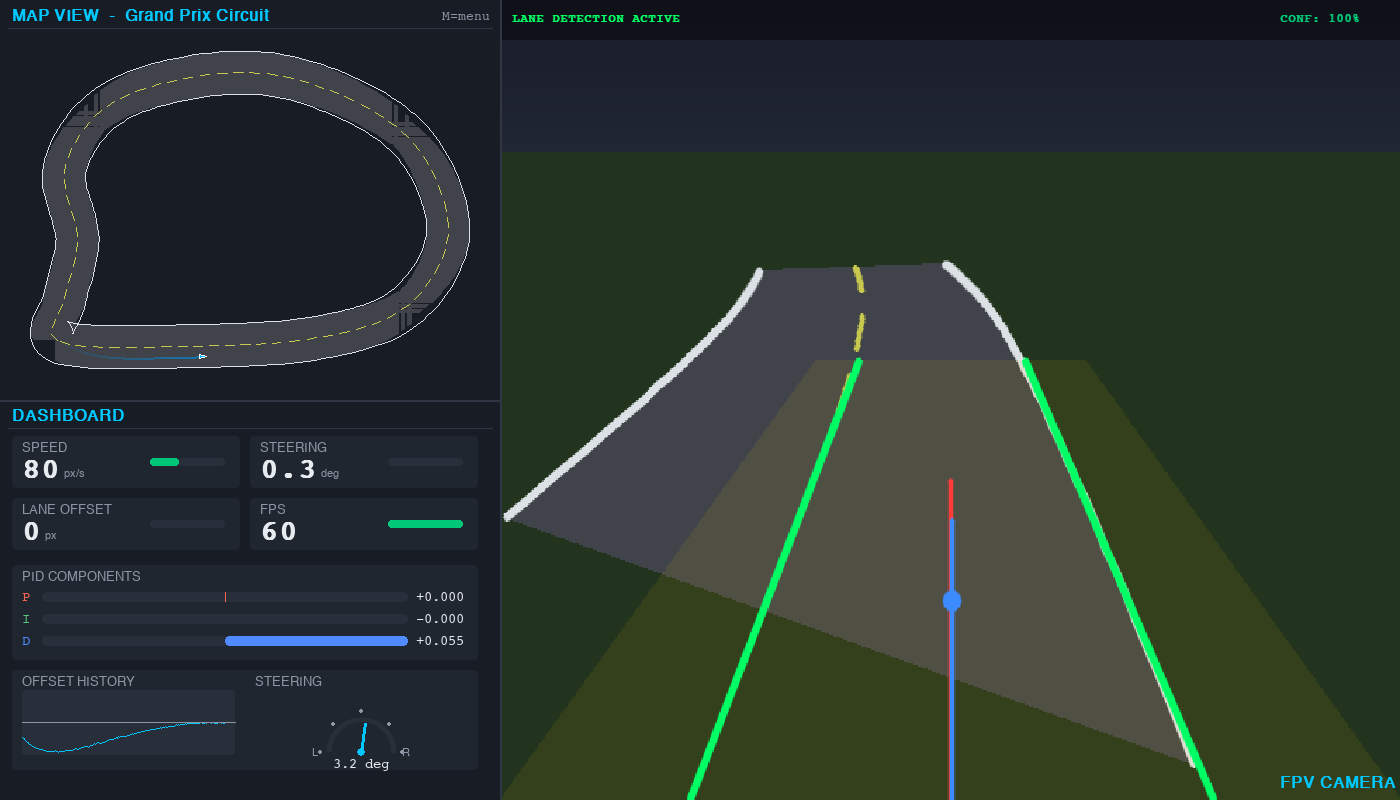
\includegraphics[width=\linewidth]{../docs/track_grand_prix.png}
    \end{column}
  \end{columns}
\end{frame}

\begin{frame}{Vehicle model: bicycle kinematics}
  \begin{columns}[T,onlytextwidth]
    \begin{column}{0.48\textwidth}
      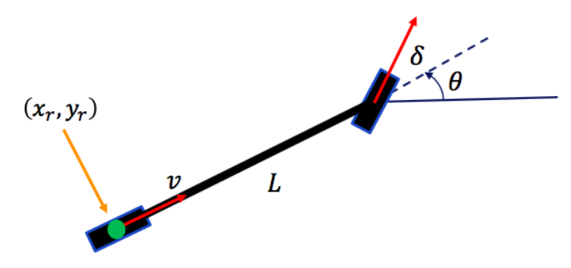
\includegraphics[width=\linewidth]{../docs/bicycle_kinematics.png}\\[4pt]
      {\footnotesize\color{gray}Rear-axle reference point $(x_r,y_r)$,
        forward speed $v$, wheelbase $L$, heading $\theta$, front-wheel
        steering angle $\delta$.}
    \end{column}
    \begin{column}{0.50\textwidth}
      Continuous-time kinematics integrated each frame:
      \[
        \begin{aligned}
          \dot{x}_r      &= v\cos\theta \\
          \dot{y}_r      &= v\sin\theta \\
          \dot{\theta}   &= \frac{v}{L}\tan\delta
        \end{aligned}
      \]
      \footnotesize
      \begin{itemize}\setlength\itemsep{1pt}
        \item Front-wheel steering, rear-axle reference -- the standard
              simplification for lane-keeping work.
        \item $\delta$ clamped to $\pm 40^\circ$; $\Delta t$ capped at
              $50$\,ms to keep the Euler integration stable.
        \item No slip, no tire model -- realistic enough for highway-
              speed lane keeping, deliberately simple so the comparison
              is about perception, not dynamics.
      \end{itemize}
    \end{column}
  \end{columns}
\end{frame}

\begin{frame}{Ground truth = analytical}
  Because we own the simulator, we can compute the things a benchmark
  is normally missing:
  \begin{itemize}\setlength\itemsep{1pt}
    \item \highlight{True lateral offset} from the centreline spline.
    \item \highlight{True heading error} vs.\ the track tangent.
    \item \highlight{True curvature} ahead (adaptive speed control,
          turn-sharpness grouping).
    \item \highlight{Ground-truth lane polygon} in the camera frame
          (re-project road from spline) $\Rightarrow$
          \highlight{lane-IoU} against any predicted mask.
  \end{itemize}
  $\Rightarrow$ Every metric is anchored to a number the detector
  \emph{cannot see}.
\end{frame}

% ════════════════════════════════════════════════════════════════════
\section{Three lane detectors}
% ════════════════════════════════════════════════════════════════════

\begin{frame}{Method 1: centroid (our baseline)}
  \begin{columns}[T,onlytextwidth]
    \begin{column}{0.55\textwidth}
      \textbf{Pipeline}
      \begin{enumerate}\setlength\itemsep{1pt}
        \item Threshold the grey road colour in HSV.
        \item Mask to a trapezoidal ROI.
        \item Centroid of the blob (image moments).
        \item EMA smoothing across frames.
      \end{enumerate}

      \vspace{0.5em}
      \textbf{Role}
      \begin{itemize}\setlength\itemsep{1pt}
        \item Simplest detector we could write $\Rightarrow$ adopted as
              the \highlight{reference baseline}.
        \item Tells us how much the lane-line geometry of Methods 2--3
              actually buys.
      \end{itemize}
    \end{column}
    \begin{column}{0.43\textwidth}
      \begin{block}{Spoiler}
        \highlight{Does not complete a lap on any track.}\\
        The blob centroid drifts off-centre whenever the road is
        asymmetric in the field of view.
      \end{block}
    \end{column}
  \end{columns}
\end{frame}

\begin{frame}{Method 2: Hough lines (the textbook pipeline)}
  \begin{columns}[T,onlytextwidth]
    \begin{column}{0.55\textwidth}
      \textbf{Pipeline}
      \begin{enumerate}\setlength\itemsep{2pt}
        \item Blur, then Canny edges.
        \item Trapezoidal ROI -- keep only the road.
        \item Probabilistic Hough $\Rightarrow$ line segments.
        \item Split by slope sign: left vs.\ right lane.
        \item Length-weighted average $\Rightarrow$ one line per side.
        \item Lane centre = midpoint at the bottom.
      \end{enumerate}
    \end{column}
    \begin{column}{0.43\textwidth}
      \textbf{Strength}
      \begin{itemize}\setlength\itemsep{1pt}
        \item Fast, no training, fully interpretable.
        \item Rock-solid on straight road.
      \end{itemize}
      \vspace{0.5em}
      \textbf{Weakness}
      \begin{itemize}\setlength\itemsep{1pt}
        \item \highlight{Models every lane as a straight line.}
        \item In a curve, the line cuts the corner -- the error grows
              with the bend.
      \end{itemize}
    \end{column}
  \end{columns}
\end{frame}

\begin{frame}{Method 3: bird's-eye + sliding-window polyfit}
  \begin{center}
    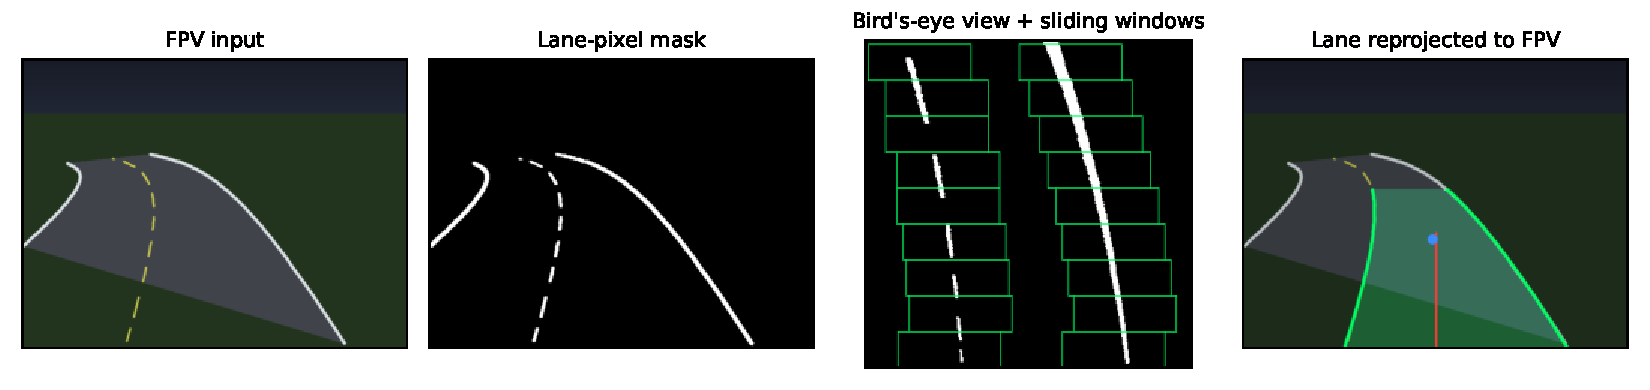
\includegraphics[width=0.94\linewidth]{figures/polyfit_pipeline.pdf}
  \end{center}
  \footnotesize
  Four stages, each fixing a specific weakness of Method 2:
  \begin{itemize}\setlength\itemsep{1pt}
    \item \highlight{Lane pixels} -- colour $+$ edges, not just Canny.
    \item \highlight{Bird's-eye warp} -- the model sees true road shape.
    \item \highlight{Sliding windows} -- robust on dashed lines.
    \item \highlight{Quadratic fit} -- a curve, not a straight line.
  \end{itemize}
\end{frame}

\begin{frame}{Method 3, step 1 -- undo the perspective}
  \begin{columns}[T,onlytextwidth]
    \begin{column}{0.55\textwidth}
      \footnotesize
      \textbf{Problem.} In the camera image, the same physical dash
      covers $\sim 30$\,px near the car but only $\sim 2$\,px far ahead.
      A pixel-counting curve fit therefore listens to the near road and
      \highlight{ignores the far field} -- exactly the part that
      announces upcoming curves.
      \vspace{0.6em}

      \textbf{Fix.} A fixed homography warps the ROI trapezoid into a
      square top-down view. In that view:
      \begin{itemize}\setlength\itemsep{1pt}
        \item Every dash is the same size, near or far.
        \item Curved lanes become \highlight{gentle bends}, not
              vanishing-point lines.
        \item A 2nd-order polynomial $x = a y^2 + b y + c$ fits a
              typical road curve almost exactly.
      \end{itemize}
    \end{column}
    \begin{column}{0.43\textwidth}\footnotesize
      \begin{block}{Why this is the key step}
        Without the warp, even a quadratic fit barely beats Hough,
        because the near road still dominates.\\[3pt]
        With the warp, near and far pixels get \highlight{equal say}
        in the fit.
      \end{block}
    \end{column}
  \end{columns}
\end{frame}

\begin{frame}{Method 3, step 2 -- find each lane}
  \footnotesize
  Inside the bird's-eye view, which pixels belong to the left vs.\
  right lane?
  \vspace{0.4em}

  \textbf{Sliding-window search}
  \begin{enumerate}\setlength\itemsep{1pt}
    \item \highlight{Seed}: column histogram of the bottom half
          $\Rightarrow$ two strongest peaks = lane bases.
    \item \highlight{Walk upward}: stack of 9 rectangular windows above
          each base; collect bright pixels inside.
    \item \highlight{Recentre}: if enough pixels are found, slide the
          next window over to follow them. Robust to dashed lines and
          short gaps.
  \end{enumerate}

  \vspace{0.4em}
  \textbf{Quadratic fit + reprojection}
  \begin{itemize}\setlength\itemsep{1pt}
    \item Least-squares fit $x = a y^2 + b y + c$ on the collected
          pixels, one polynomial per lane.
    \item EMA on the coefficients $\Rightarrow$ stable across frames.
    \item Warp the curve back to the camera image for the overlay and
          for the lane-IoU metric.
  \end{itemize}
\end{frame}

\begin{frame}{Method 3, step 3 -- the look-ahead offset}
  \begin{columns}[T,onlytextwidth]
    \begin{column}{0.5\textwidth}
      \begin{itemize}\setlength\itemsep{1pt}
        \item The polynomial gives us the lane \emph{shape}, not just
              one point on it.
        \item Evaluate the lane centre at \highlight{45\,\% up the
              BEV} -- a 1-frame predictor, essentially free.
        \item Feed \emph{that} to the PID instead of the bottom-of-
              image offset.
        \item Turn it off and the polyfit's RMS gain shrinks from
              $\sim 40\,\%$ to $\sim 10\,\%$.
      \end{itemize}
    \end{column}
    \begin{column}{0.48\textwidth}
      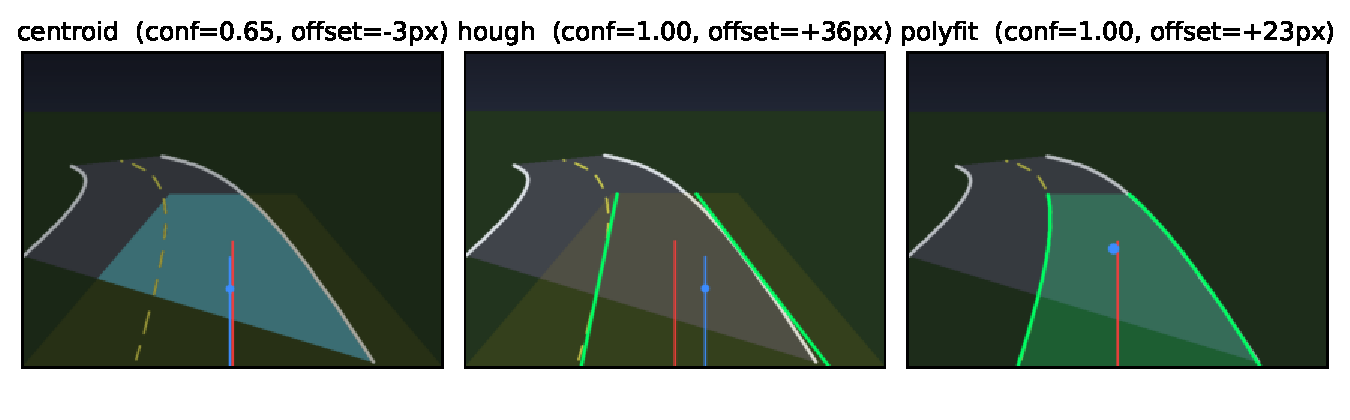
\includegraphics[width=\linewidth]{figures/annotations.pdf}\\
      {\footnotesize\color{gray}The blue dot in the right panel is the
        reprojected look-ahead point.}
    \end{column}
  \end{columns}
\end{frame}

% ════════════════════════════════════════════════════════════════════
\section{Two controllers}
% ════════════════════════════════════════════════════════════════════

\begin{frame}{PID -- the baseline controller}
  \[
    \delta_t = K_p\,e_t
              + K_i\!\sum_{\tau\le t}\!e_\tau\,\Delta t
              + K_d\,\dot e_t
  \]
  \begin{itemize}
    \item Input: normalised lateral offset $e\in[-1,+1]$ from the
          detector.
    \item Gains tuned by hand on the oval:
          $K_p=1.2,\;K_i=0.008,\;K_d=0.5$.
    \item Integral anti-windup at $\pm 50$.
    \item Reactive only -- has no model of the path.
  \end{itemize}
\end{frame}

\begin{frame}{Stanley -- the perception-free oracle}
  \[
    \delta = \psi + \arctan\!\Bigl(\tfrac{k\,e_\perp}{k_s + v}\Bigr)
  \]
  \begin{itemize}
    \item Heading error $\psi$ + cross-track error $e_\perp$ at the
          front axle, both computed from the \emph{true} spline.
    \item Gains $k=0.6$, $k_s=20$.
    \item \highlight{It does not look at the camera.}
    \item Result on every track: $<1$\,px RMS lateral error.
    \item Interpretation: the gap between PID-on-detection and
          Stanley-on-truth is \emph{purely} the perception error.
  \end{itemize}
\end{frame}

% ════════════════════════════════════════════════════════════════════
\section{Experiments}
% ════════════════════════════════════════════════════════════════════

\begin{frame}{Headline result: RMS lateral error per track}
  \vspace{-0.5em}
  \begin{center}
    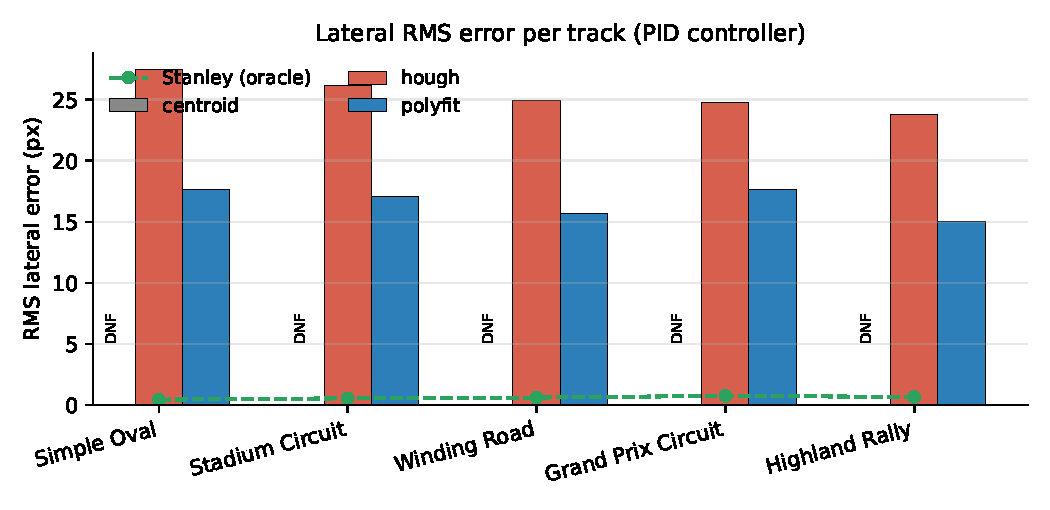
\includegraphics[width=0.78\linewidth]{figures/rms_by_track.pdf}
  \end{center}
  \vspace{-0.6em}
  \footnotesize Centroid \highlight{DNF} on every track. On the
  $5$ base tracks: Hough $25.4$\,px mean RMS, polyfit
  $\mathbf{16.6}$\,px ($\highlight{-34\,\%}$). Red Bull Ring (hairpins,
  adaptive speed): \highlight{polyfit DNFs} at a hairpin, Hough
  survives at $31.0$\,px. Stanley+truth: $<2$\,px throughout.
\end{frame}

\begin{frame}{The full table}
  \vspace{-0.4em}
  \begin{center}\tiny\setlength{\tabcolsep}{4pt}
    \renewcommand{\arraystretch}{0.9}
    \begin{tabular}{l l r r r r r r}
\toprule
Track & Detector & Lap & RMS px & Mean px & Max px & IoU & ms/det \\
\midrule
Simple Oval & centroid & DNF & 99.5 & 80.0 & 194.3 & 0.01 & 1.15 \\
Simple Oval & hough & \checkmark & 27.4 & 27.2 & 28.7 & 0.17 & 0.75 \\
Simple Oval & polyfit & \checkmark & 17.6 & 16.9 & 27.2 & 0.25 & 1.92 \\
\midrule
Stadium Circuit & centroid & DNF & 39.5 & 32.8 & 113.4 & 0.39 & 1.79 \\
Stadium Circuit & hough & \checkmark & 26.2 & 26.0 & 30.1 & 0.24 & 0.77 \\
Stadium Circuit & polyfit & \checkmark & 17.0 & 16.3 & 23.6 & 0.31 & 1.94 \\
\midrule
Winding Road & centroid & DNF & 33.9 & 28.2 & 97.8 & 0.41 & 1.84 \\
Winding Road & hough & \checkmark & 24.9 & 24.7 & 28.4 & 0.23 & 0.76 \\
Winding Road & polyfit & \checkmark & 15.7 & 14.8 & 23.7 & 0.35 & 1.96 \\
\midrule
Grand Prix Circuit & centroid & DNF & 35.0 & 28.4 & 108.4 & 0.43 & 1.91 \\
Grand Prix Circuit & hough & \checkmark & 24.8 & 24.6 & 27.8 & 0.26 & 0.77 \\
Grand Prix Circuit & polyfit & \checkmark & 17.7 & 16.1 & 34.5 & 0.36 & 1.95 \\
\midrule
Highland Rally & centroid & DNF & 65.6 & 52.9 & 127.6 & 0.00 & 1.22 \\
Highland Rally & hough & \checkmark & 23.8 & 23.6 & 26.1 & 0.31 & 0.78 \\
Highland Rally & polyfit & \checkmark & 15.1 & 14.2 & 21.9 & 0.39 & 1.95 \\
\midrule
Red Bull Ring & centroid & DNF & 117.7 & 95.0 & 228.4 & 0.01 & 1.12 \\
Red Bull Ring & hough & \checkmark & 31.0 & 30.5 & 51.9 & 0.21 & 0.73 \\
Red Bull Ring & polyfit & DNF & 28.5 & 22.8 & 82.0 & 0.24 & 1.90 \\
\midrule
Simple Oval & Stanley (oracle) & \checkmark & 0.4 & 0.4 & 1.2 & 0.52 & 2.04 \\
\bottomrule
\end{tabular}
  \end{center}
  \vspace{-0.2em}
  \scriptsize
  \begin{itemize}\setlength\itemsep{0pt}
    \item Where polyfit completes, it beats Hough on RMS and IoU
          ($-34\,\%$ RMS, $+38\,\%$ IoU averaged).
    \item \highlight{Red Bull Ring caveat}: the quadratic fit briefly
          blows up at a hairpin and the car leaves the road. Hough's
          straight line degrades gracefully and finishes.
  \end{itemize}
\end{frame}

\begin{frame}{Red Bull Ring: where polyfit falls over}
  \vspace{-0.5em}
  \begin{center}
    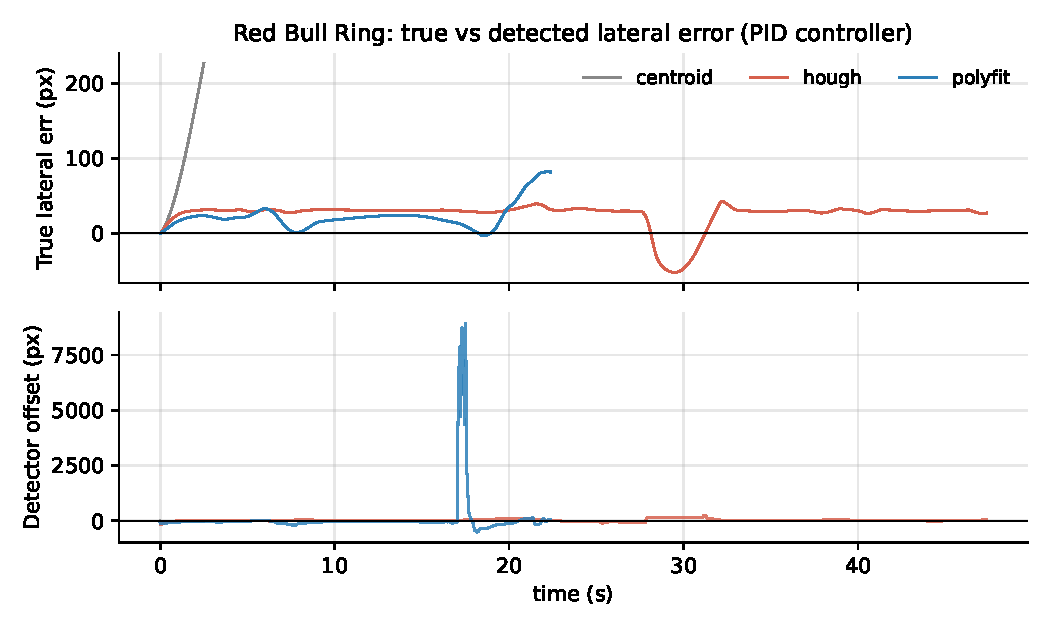
\includegraphics[width=0.70\linewidth]{figures/redbull_ring_traces.pdf}
  \end{center}
  \vspace{-0.5em}
  \scriptsize \highlight{Top:} centroid bails at $t\!\approx\!3$\,s.
  Hough holds $\sim 30$\,px to the flag. Polyfit trails Hough until
  $t\!\approx\!17$\,s.\\
  \highlight{Bottom:} a hairpin makes the quadratic fit explode to
  $\sim\!8000$\,px for two frames -- PID over-corrects, car off-track.
  \highlight{Fix:} clamp detector offset, or reject fit outliers.
\end{frame}

\begin{frame}{Robustness to camera noise}
  \begin{columns}[T,onlytextwidth]
    \begin{column}{0.55\textwidth}
      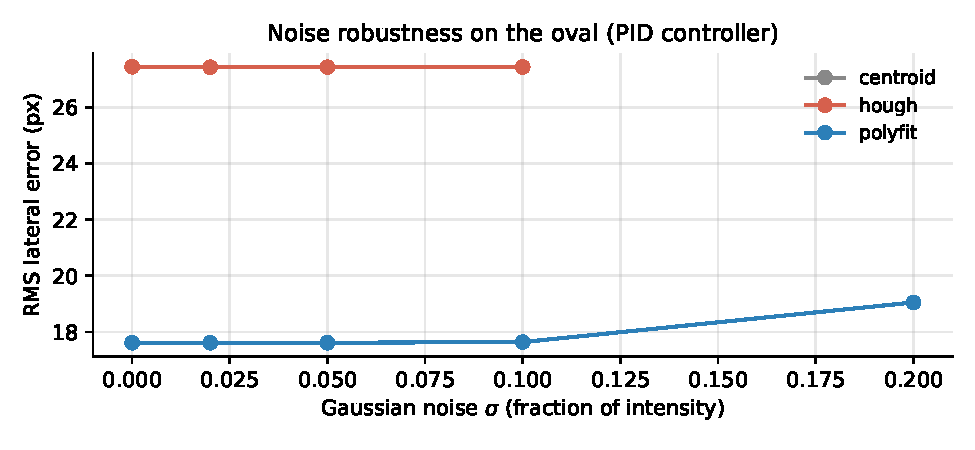
\includegraphics[width=\linewidth]{figures/noise.pdf}
    \end{column}
    \begin{column}{0.43\textwidth}\footnotesize
      \begin{itemize}\setlength\itemsep{1pt}
        \item Same oval, PID, $+$Gaussian noise
              $\sigma\in[0,0.20]$ per frame.
        \item Centroid never completes.
        \item Hough survives $\sigma\le 0.10$, fails at $0.20$
              (Canny drowned out).
        \item \highlight{Polyfit completes at every $\sigma$} -- its
              mask uses a \emph{normalised} Sobel-x + colour.
      \end{itemize}
    \end{column}
  \end{columns}
\end{frame}

\begin{frame}{Compute cost}
  \begin{center}
    \begin{tabular}{lrr}
      \toprule
      Detector & ms / frame & equiv.\ FPS \\
      \midrule
      centroid & 1.7 & $\sim$600 \\
      hough    & 0.7 & $\sim$1450 \\
      polyfit  & 1.9 & $\sim$520 \\
      \bottomrule
    \end{tabular}
  \end{center}
  \vspace{1em}
  \begin{itemize}
    \item All three are comfortably real-time on a single CPU thread.
    \item Polyfit overhead is dominated by the perspective warp and
          \code{np.polyfit}, not by the sliding-window scan.
    \item Plenty of budget left for downstream tasks (other vehicles,
          obstacles, signs).
  \end{itemize}
\end{frame}

% ════════════════════════════════════════════════════════════════════
\section{Live demo}
% ════════════════════════════════════════════════════════════════════

\begin{frame}{Live demo}
  \begin{center}\large
    \texttt{python main.py {-}{-}detector polyfit {-}{-}controller pid}
  \end{center}
  \vspace{1em}
  \begin{itemize}
    \item Press \highlight{D} to cycle detectors live.
    \item Press \highlight{C} to toggle PID $\leftrightarrow$ Stanley.
    \item Press \highlight{M} to jump back to the track selector.
    \item Watch the dashboard: lane offset, FPS, PID components.
  \end{itemize}
  \vspace{1em}
  Suggested demo route: \emph{Stadium} (Hough wobbles) $\to$
  \emph{Winding Road} (Hough struggles) $\to$ switch to polyfit
  $\to$ switch to Stanley.
\end{frame}

% ════════════════════════════════════════════════════════════════════
\section{Discussion and conclusion}
% ════════════════════════════════════════════════════════════════════

\begin{frame}{What worked, what failed}
  \footnotesize
  \begin{block}{Worked}
    \begin{itemize}\setlength\itemsep{0pt}
      \item Look-ahead offset = single biggest gain.
      \item HSV + Sobel mask cleaner than Canny on dashed lines.
      \item Quadratic fits + EMA give stable curves.
    \end{itemize}
  \end{block}
  \begin{alertblock}{Failed / limitations}
    \begin{itemize}\setlength\itemsep{0pt}
      \item Centroid is structurally biased -- no tuning saves it.
      \item Hough lingers on its last good line through tight bends.
      \item Polyfit's quadratic fit can \highlight{blow up at tight
            hairpins} (Red Bull Ring) -- needs outlier rejection.
      \item IPM warp assumes flat ground; real cameras need re-tuning.
      \item Simulator is too clean -- numbers are an upper bound.
    \end{itemize}
  \end{alertblock}
\end{frame}

\begin{frame}{Take-aways}
  \begin{itemize}
    \item A modest classical-CV upgrade (BEV warp + sliding-window
          quadratic fit) cuts RMS lateral error by \highlight{34--40\,\%}
          vs.\ the textbook Hough pipeline.
    \item The change is fully interpretable: we can point at each
          stage in Fig.~3 and say why it helps.
    \item Look-ahead offsets are essentially free on top of a
          polynomial fit and turn a reactive PID into a quasi-MPC.
    \item Closing the remaining gap to Stanley-on-truth would need
          sub-pixel-accurate perception $\Rightarrow$ a learned
          segmenter is the next step.
  \end{itemize}
\end{frame}

\begin{frame}[standout]
  Thank you. \\[2em]
  \small\color{gray}
  Code, simulator, report and these slides are all in this repo.\\
  Questions?
\end{frame}

\appendix

\begin{frame}{Backup: detector confidence per track}
  \begin{itemize}
    \item Centroid mean confidence: \highlight{0.27} (HSV blob coverage,
          near zero whenever the road leaves the trapezoid).
    \item Hough mean confidence: \highlight{0.99} (both lines almost
          always found -- but ``found'' $\ne$ ``correct'').
    \item Polyfit mean confidence: \highlight{1.00} (both polynomial
          fits valid in every frame after warm-up).
    \item Take-away: high detector confidence does not imply low
          error. Lane-IoU is the better proxy.
  \end{itemize}
\end{frame}

\begin{frame}{Backup: why the look-ahead works}
  Recall the bicycle heading update:
  \[
    \dot\theta = \frac{v}{L}\tan\delta
  \]
  \begin{itemize}
    \item A pure-P controller on $e_\text{bottom}$ reacts to
          \emph{current} position only.
    \item Adding the look-ahead error $e_\text{LA}$ effectively
          augments the controller with a free derivative term that
          knows where the road is going.
    \item Equivalent to a one-step preview MPC with horizon
          $\sim 0.5$\,s at typical speeds -- without solving an
          optimisation.
  \end{itemize}
\end{frame}

\begin{frame}{Backup: reproducibility}
  \begin{center}\footnotesize\ttfamily
    git clone <repo>\\
    python -m venv .venv \&\& source .venv/bin/activate\\
    pip install -r requirements.txt matplotlib pdf2image\\
    python experiments.py \quad\# CSVs + summary figures\\
    python make\_qualitative\_figures.py \quad\# overlays\\
    cd presentation \&\& tectonic report.tex\\
    cd presentation \&\& tectonic slides.tex
  \end{center}
  \vspace{0.6em}
  \small All experiments are deterministic except the noise sweep,
  seeded by NumPy's default RNG.
\end{frame}

\end{document}
